% Options for packages loaded elsewhere
\PassOptionsToPackage{unicode}{hyperref}
\PassOptionsToPackage{hyphens}{url}
%
\documentclass[
]{article}
\usepackage{lmodern}
\usepackage{amsmath}
\usepackage{ifxetex,ifluatex}
\ifnum 0\ifxetex 1\fi\ifluatex 1\fi=0 % if pdftex
  \usepackage[T1]{fontenc}
  \usepackage[utf8]{inputenc}
  \usepackage{textcomp} % provide euro and other symbols
  \usepackage{amssymb}
\else % if luatex or xetex
  \usepackage{unicode-math}
  \defaultfontfeatures{Scale=MatchLowercase}
  \defaultfontfeatures[\rmfamily]{Ligatures=TeX,Scale=1}
\fi
% Use upquote if available, for straight quotes in verbatim environments
\IfFileExists{upquote.sty}{\usepackage{upquote}}{}
\IfFileExists{microtype.sty}{% use microtype if available
  \usepackage[]{microtype}
  \UseMicrotypeSet[protrusion]{basicmath} % disable protrusion for tt fonts
}{}
\makeatletter
\@ifundefined{KOMAClassName}{% if non-KOMA class
  \IfFileExists{parskip.sty}{%
    \usepackage{parskip}
  }{% else
    \setlength{\parindent}{0pt}
    \setlength{\parskip}{6pt plus 2pt minus 1pt}}
}{% if KOMA class
  \KOMAoptions{parskip=half}}
\makeatother
\usepackage{xcolor}
\IfFileExists{xurl.sty}{\usepackage{xurl}}{} % add URL line breaks if available
\IfFileExists{bookmark.sty}{\usepackage{bookmark}}{\usepackage{hyperref}}
\hypersetup{
  pdftitle={R-Bootcamp Report},
  pdfauthor={Leonid Gavrilyuk; Bernardo Freire Barboza da Cruz},
  hidelinks,
  pdfcreator={LaTeX via pandoc}}
\urlstyle{same} % disable monospaced font for URLs
\usepackage[margin=1in]{geometry}
\usepackage{longtable,booktabs}
\usepackage{calc} % for calculating minipage widths
% Correct order of tables after \paragraph or \subparagraph
\usepackage{etoolbox}
\makeatletter
\patchcmd\longtable{\par}{\if@noskipsec\mbox{}\fi\par}{}{}
\makeatother
% Allow footnotes in longtable head/foot
\IfFileExists{footnotehyper.sty}{\usepackage{footnotehyper}}{\usepackage{footnote}}
\makesavenoteenv{longtable}
\usepackage{graphicx}
\makeatletter
\def\maxwidth{\ifdim\Gin@nat@width>\linewidth\linewidth\else\Gin@nat@width\fi}
\def\maxheight{\ifdim\Gin@nat@height>\textheight\textheight\else\Gin@nat@height\fi}
\makeatother
% Scale images if necessary, so that they will not overflow the page
% margins by default, and it is still possible to overwrite the defaults
% using explicit options in \includegraphics[width, height, ...]{}
\setkeys{Gin}{width=\maxwidth,height=\maxheight,keepaspectratio}
% Set default figure placement to htbp
\makeatletter
\def\fps@figure{htbp}
\makeatother
\setlength{\emergencystretch}{3em} % prevent overfull lines
\providecommand{\tightlist}{%
  \setlength{\itemsep}{0pt}\setlength{\parskip}{0pt}}
\setcounter{secnumdepth}{5}
\ifluatex
  \usepackage{selnolig}  % disable illegal ligatures
\fi

\title{R-Bootcamp Report}
\author{Leonid Gavrilyuk\footnote{Hochschule Luzern,
  \href{mailto:leonid.gavrilyuk@stud.hslu.ch}{\nolinkurl{leonid.gavrilyuk@stud.hslu.ch}}} \and Bernardo
Freire Barboza da Cruz\footnote{Hochschule Luzern,
  \href{mailto:bernardo.dacruz@stud.hslu.ch}{\nolinkurl{bernardo.dacruz@stud.hslu.ch}}}}
\date{22 February, 2022}

\begin{document}
\maketitle

\centering
\raggedright
\newpage
\tableofcontents
\pagebreak

\hypertarget{introduction}{%
\section{Introduction}\label{introduction}}

\hypertarget{project-goal}{%
\subsection{Project goal}\label{project-goal}}

The goal is to understand the dynamics in the performance of each part
in each electoral district of the city. The period of interest is
2006-2018. The questions to be answered: what is the dynamic of the
voting behaviour in each electoral district, overview of the city
elections, identification of relationship (if any) between such
characteristics as voters' education and the election results of the
party.

\hypertarget{data}{%
\subsection{Data}\label{data}}

To perform analysis, six data sets covering the time period 2006-2018
were retrieved from the Open Data platform of the City of Zürich:

\begin{itemize}
\tightlist
\item
  Turnout at the city and municipal council elections, by city district,
  since 2006.
\item
  Municipal elections vote share, by party and electoral district, since
  1913.
\item
  Turnout at the city and municipal council elections, by age and
  gender, since 2006.
\item
  Wealth distribution of the population in Zürich, by district, since
  1999.
\item
  Income distribution of the population in Zürich, by district, since
  1999.
\end{itemize}

The data sets did not have the same content and were not organised in
the same way. Each data set contained some irrelevant information - for
example, historical election data since 1913 whereas the time span of
interest is 2006-2018. This required data preparation activities. Each
data set was prepared, subsequently, all of them were merged into one
final table.

\pagebreak

\hypertarget{data-preparation}{%
\section{Data Preparation}\label{data-preparation}}

\hypertarget{data-set-1-turnout-at-the-city-and-municipal-council-elections-since-2006-by-city-district.}{%
\subsection{Data set 1: Turnout at the city and municipal council
elections since 2006, by city
district.}\label{data-set-1-turnout-at-the-city-and-municipal-council-elections-since-2006-by-city-district.}}

The data set of dimensions 136x7 reflects how many people from each city
district participated in the last five elections (2006-2018).

\begin{longtable}[]{@{}rrlrrrr@{}}
\caption{Original data set: Turnout in the city and municipal council
elections since 2006, by city district}\tabularnewline
\toprule
Jahr & QNr & Qname & Sberechtigte & Nteilnehmende & teilnehmende &
Beteiligung\tabularnewline
\midrule
\endfirsthead
\toprule
Jahr & QNr & Qname & Sberechtigte & Nteilnehmende & teilnehmende &
Beteiligung\tabularnewline
\midrule
\endhead
2006 & 11 & Rathaus (Kreis 1) & 1974 & 1186 & 788 & 39.9\tabularnewline
2006 & 12 & Hochschulen (Kreis 1) & 377 & 232 & 145 &
38.5\tabularnewline
2006 & 13 & Lindenhof (Kreis 1) & 1335 & 962 & 373 & 27.9\tabularnewline
2006 & 14 & City (Kreis 1) & 597 & 440 & 157 & 26.3\tabularnewline
2006 & 21 & Wollishofen (Kreis 2) & 10115 & 6168 & 3947 &
39.0\tabularnewline
2006 & 23 & Leimbach (Kreis 2) & 3123 & 1997 & 1126 &
36.1\tabularnewline
\bottomrule
\end{longtable}

Examination of the dataset revealed an important issue: The territorial
entity in this dataset is a city district - \emph{``Stadtquartier''}.
However, in Zürich, the elections are held across 12 electoral districts
- \emph{``Wahlkreise''}. Each electoral district consists of several
``Stadtquartiers''. For example, electoral district ``Kreis 1+2'' unites
six city districts (they are shown in the ``Qname'' column in the Table
1 above).

To address the issue, the following manipulations were performed:

\begin{itemize}
\tightlist
\item
  In the column ``Qname'', the electoral district is specified in the
  parentheses: e.g.~``Rathaus (Kreis 1)''. The content of the
  parentheses was extracted with the \textbf{stringr package} and stored
  in the created column ``DistrictName''.
\item
  Rename the electoral districts to reflect the fact that some city
  districts are merged for the elections - for example, ``Kreis 1'' and
  ``Kreis 2'' became ``Kreis 1+2''. This was done with the \textbf{dplyr
  mutate() function}.
\item
  Assigning levels to the DistrictNamecolumn to prevent ordering
  alphabetically: Kreis 1+2 is now followed by Kreis 3, and not Kreis
  10.
\item
  Calculate the mean values for each group and year using \textbf{dplyr
  group\_by() and summarise() functions} (saved as a separate data
  frame). The results is saved as a separate data frame, with the new
  column ``PercentageOfDistrict''.
\item
  Merge the dataframes with the \textbf{dplyr inner\_join()}.
\item
  Change ``Jahr'' and ``DistrictName'' to factors with the built-in
  \textbf{as.factor()}
\end{itemize}

\begin{longtable}[]{@{}llr@{}}
\caption{Final dataset: Turnout by electoral district}\tabularnewline
\toprule
Year & DistrictName & PercentageOfDistrict\tabularnewline
\midrule
\endfirsthead
\toprule
Year & DistrictName & PercentageOfDistrict\tabularnewline
\midrule
\endhead
2018 & Kreis 1 + 2 & 55.46\tabularnewline
2018 & Kreis 3 & 58.23\tabularnewline
2018 & Kreis 4 + 5 & 58.24\tabularnewline
2018 & Kreis 6 & 66.55\tabularnewline
2018 & Kreis 7 + 8 & 65.16\tabularnewline
2018 & Kreis 9 & 54.20\tabularnewline
\bottomrule
\end{longtable}

The analysis shows that the amount of voters in each district has grown
since 2006 - Zürich residents are becoming more active in exercising
their right to vote. Kreis 6 has the highest percentage of active
citizens, followed by Kreis 7+8 and Kreis 10. Residents of Kreis 12 are
the least interested in the elections people in Zürich. However, when it
comes to the percentage of all city voters, Kreis 12 contributes the
third largest portion of votes. This means politicians should mobilize
residents of this district to gain votes on the city and national level
elections. Other important districts are Kreis 7+8 (gives most votes)
and Kreis 11 (second place).

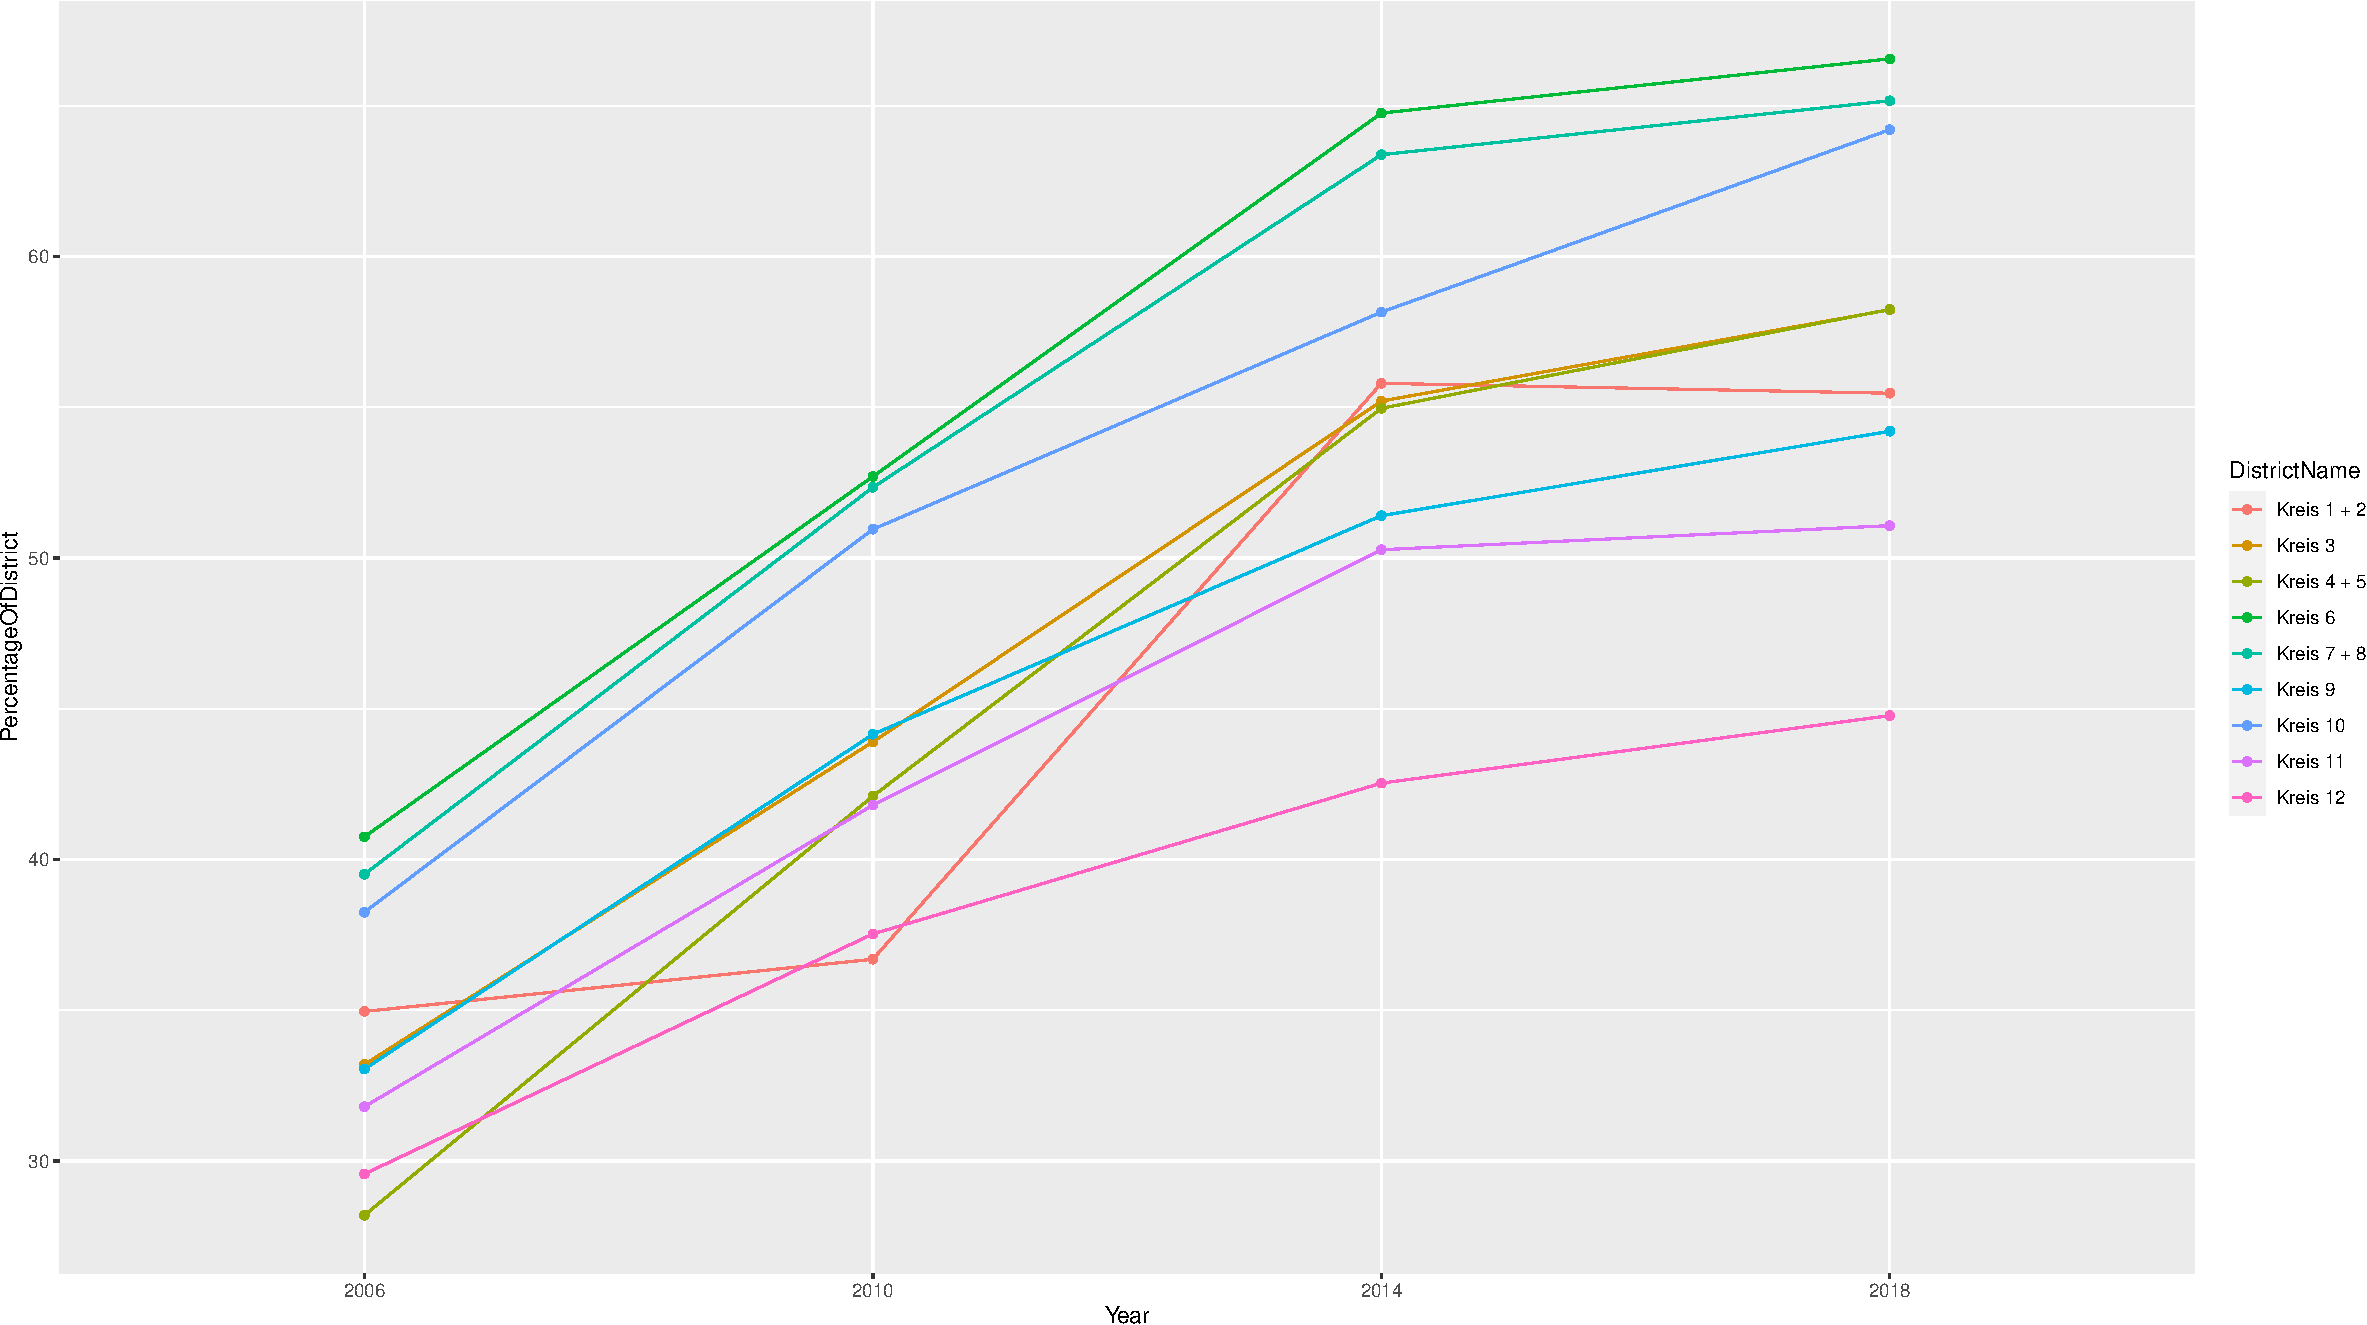
\includegraphics{report_files/figure-latex/plot_election_per_district-1.pdf}

\hypertarget{data-set-2-municipal-elections-vote-share-by-party-and-electoral-district-since-1913.}{%
\subsection{Data set 2: Municipal elections vote share, by party and
electoral district since
1913.}\label{data-set-2-municipal-elections-vote-share-by-party-and-electoral-district-since-1913.}}

The data set of dimensions 5100x6 shows the results of each party at the
elections since 1913. Naturally, it contains a lot of irrelevant
information because of the changes that happened sine 1913. For example,
for each year there are separate rows for ``Kreis 1 (before 2002)'',
``Kreis 2 (before 2002) and''Kreis 1+2 (after 2006)" - the districts
were united in 2002. Some political parties do not exist anymore; some
parties changed their names. Additionally, the table is in the long
format whereas the final data set requires it to be wide.

\begin{longtable}[]{@{}rlrlrr@{}}
\caption{Original data set: Municipal elections vote share, by party and
electoral district since 1913.}\tabularnewline
\toprule
Jahr & Partei & ParteiNr & Wahlkreis & WahlkreisSort &
Stimmenanteil\tabularnewline
\midrule
\endfirsthead
\toprule
Jahr & Partei & ParteiNr & Wahlkreis & WahlkreisSort &
Stimmenanteil\tabularnewline
\midrule
\endhead
1913 & SP & 1 & Stadt Zürich & 0 & 39.1\tabularnewline
1913 & BGB/SVP & 2 & Stadt Zürich & 0 & NA\tabularnewline
1913 & FDP & 3 & Stadt Zürich & 0 & 38.6\tabularnewline
1913 & GPS & 4 & Stadt Zürich & 0 & NA\tabularnewline
1913 & GLP & 5 & Stadt Zürich & 0 & NA\tabularnewline
1913 & CVP/Die Mitte & 6 & Stadt Zürich & 0 & 7.9\tabularnewline
\bottomrule
\end{longtable}

The following manipulations were performed:

\begin{itemize}
\tightlist
\item
  Choose only relevant time period (years 2006-2018) and eight still
  existing parties using the \textbf{\%in\% operator}.
\item
  Change the names of the electoral districts. For example, ``Kreis 11
  (ab 1974)'' became simply ``Kreis 11'' - the content in the
  parentheses was removed with the \textbf{stringr str\_replace()
  function}.
\item
  Rename the columns with the \textbf{dplyr \%\textgreater\% rename()
  function} to keep them in line with the other tables
  (e.g.~``Wahlkreis'' to ``DistrictName'').
\item
  Remove unnecessary columns with the \textbf{dplyr \%\textgreater\%
  select() function}.
\item
  Transform the table into wide format with the \textbf{tidyverse
  pivot\_wider() function}.
\item
  Change ``Year'' and ``DistrictName'' variables to factors. Visualise
  with the \textbf{tidyverse gather() method and ggplot}
\item
  Merge the set with the first table ``Turnout by electoral district''
  (see part 2.1.) using \textbf{inner\_join}.
\end{itemize}

\begin{longtable}[]{@{}llrrrrrrrr@{}}
\caption{Final dataset: Municipal elections vote share, by party and
electoral district, 2006-2018.}\tabularnewline
\toprule
Year & DistrictName & SP & BGB/SVP & FDP & GPS & GLP & CVP/Die Mitte &
AL & EVP\tabularnewline
\midrule
\endfirsthead
\toprule
Year & DistrictName & SP & BGB/SVP & FDP & GPS & GLP & CVP/Die Mitte &
AL & EVP\tabularnewline
\midrule
\endhead
2006 & Kreis 1 + 2 & 30.1 & 16.2 & 23.1 & 13.1 & 2.4 & 7.7 & 2.5 &
3.0\tabularnewline
2010 & Kreis 1 + 2 & 28.0 & 16.9 & 19.3 & 13.7 & 8.6 & 5.8 & 2.6 &
1.9\tabularnewline
2014 & Kreis 1 + 2 & 26.6 & 16.2 & 21.0 & 11.4 & 10.5 & 5.1 & 4.9 &
1.9\tabularnewline
2018 & Kreis 1 + 2 & 30.8 & 13.1 & 19.8 & 12.4 & 10.4 & 4.3 & 6.3 &
1.5\tabularnewline
2006 & Kreis 3 & 37.5 & 18.2 & 8.6 & 14.3 & 2.3 & 7.1 & 6.1 &
2.3\tabularnewline
2010 & Kreis 3 & 34.2 & 16.9 & 8.1 & 13.5 & 10.4 & 5.1 & 6.9 &
1.7\tabularnewline
2014 & Kreis 3 & 32.1 & 15.0 & 10.5 & 12.8 & 10.4 & 4.0 & 9.8 &
1.4\tabularnewline
2018 & Kreis 3 & 35.8 & 10.3 & 10.9 & 14.1 & 10.4 & 3.2 & 12.1 &
1.6\tabularnewline
\bottomrule
\end{longtable}

The visualisation shows that parties have been demonstrating roughly the
same result since 2006. Kreis 7+8 seems to be the bastion of FDP. Most
active supporters of AL-Alternative Liste live in Kreis 4+5. Electoral
districts Kreis 3, Kreis 4+5, Kreis 6 and Kreis 10 deliver a larger
amount of votes to SP than the citizens of other districts. Voters in
Kreis 7+8 do not like to vote for socialists. A curious phenomenon can
be observed when it comes to the green parties - GLP and GPS. They seem
to grow at expense of other parties: FDP and SP, respectively.

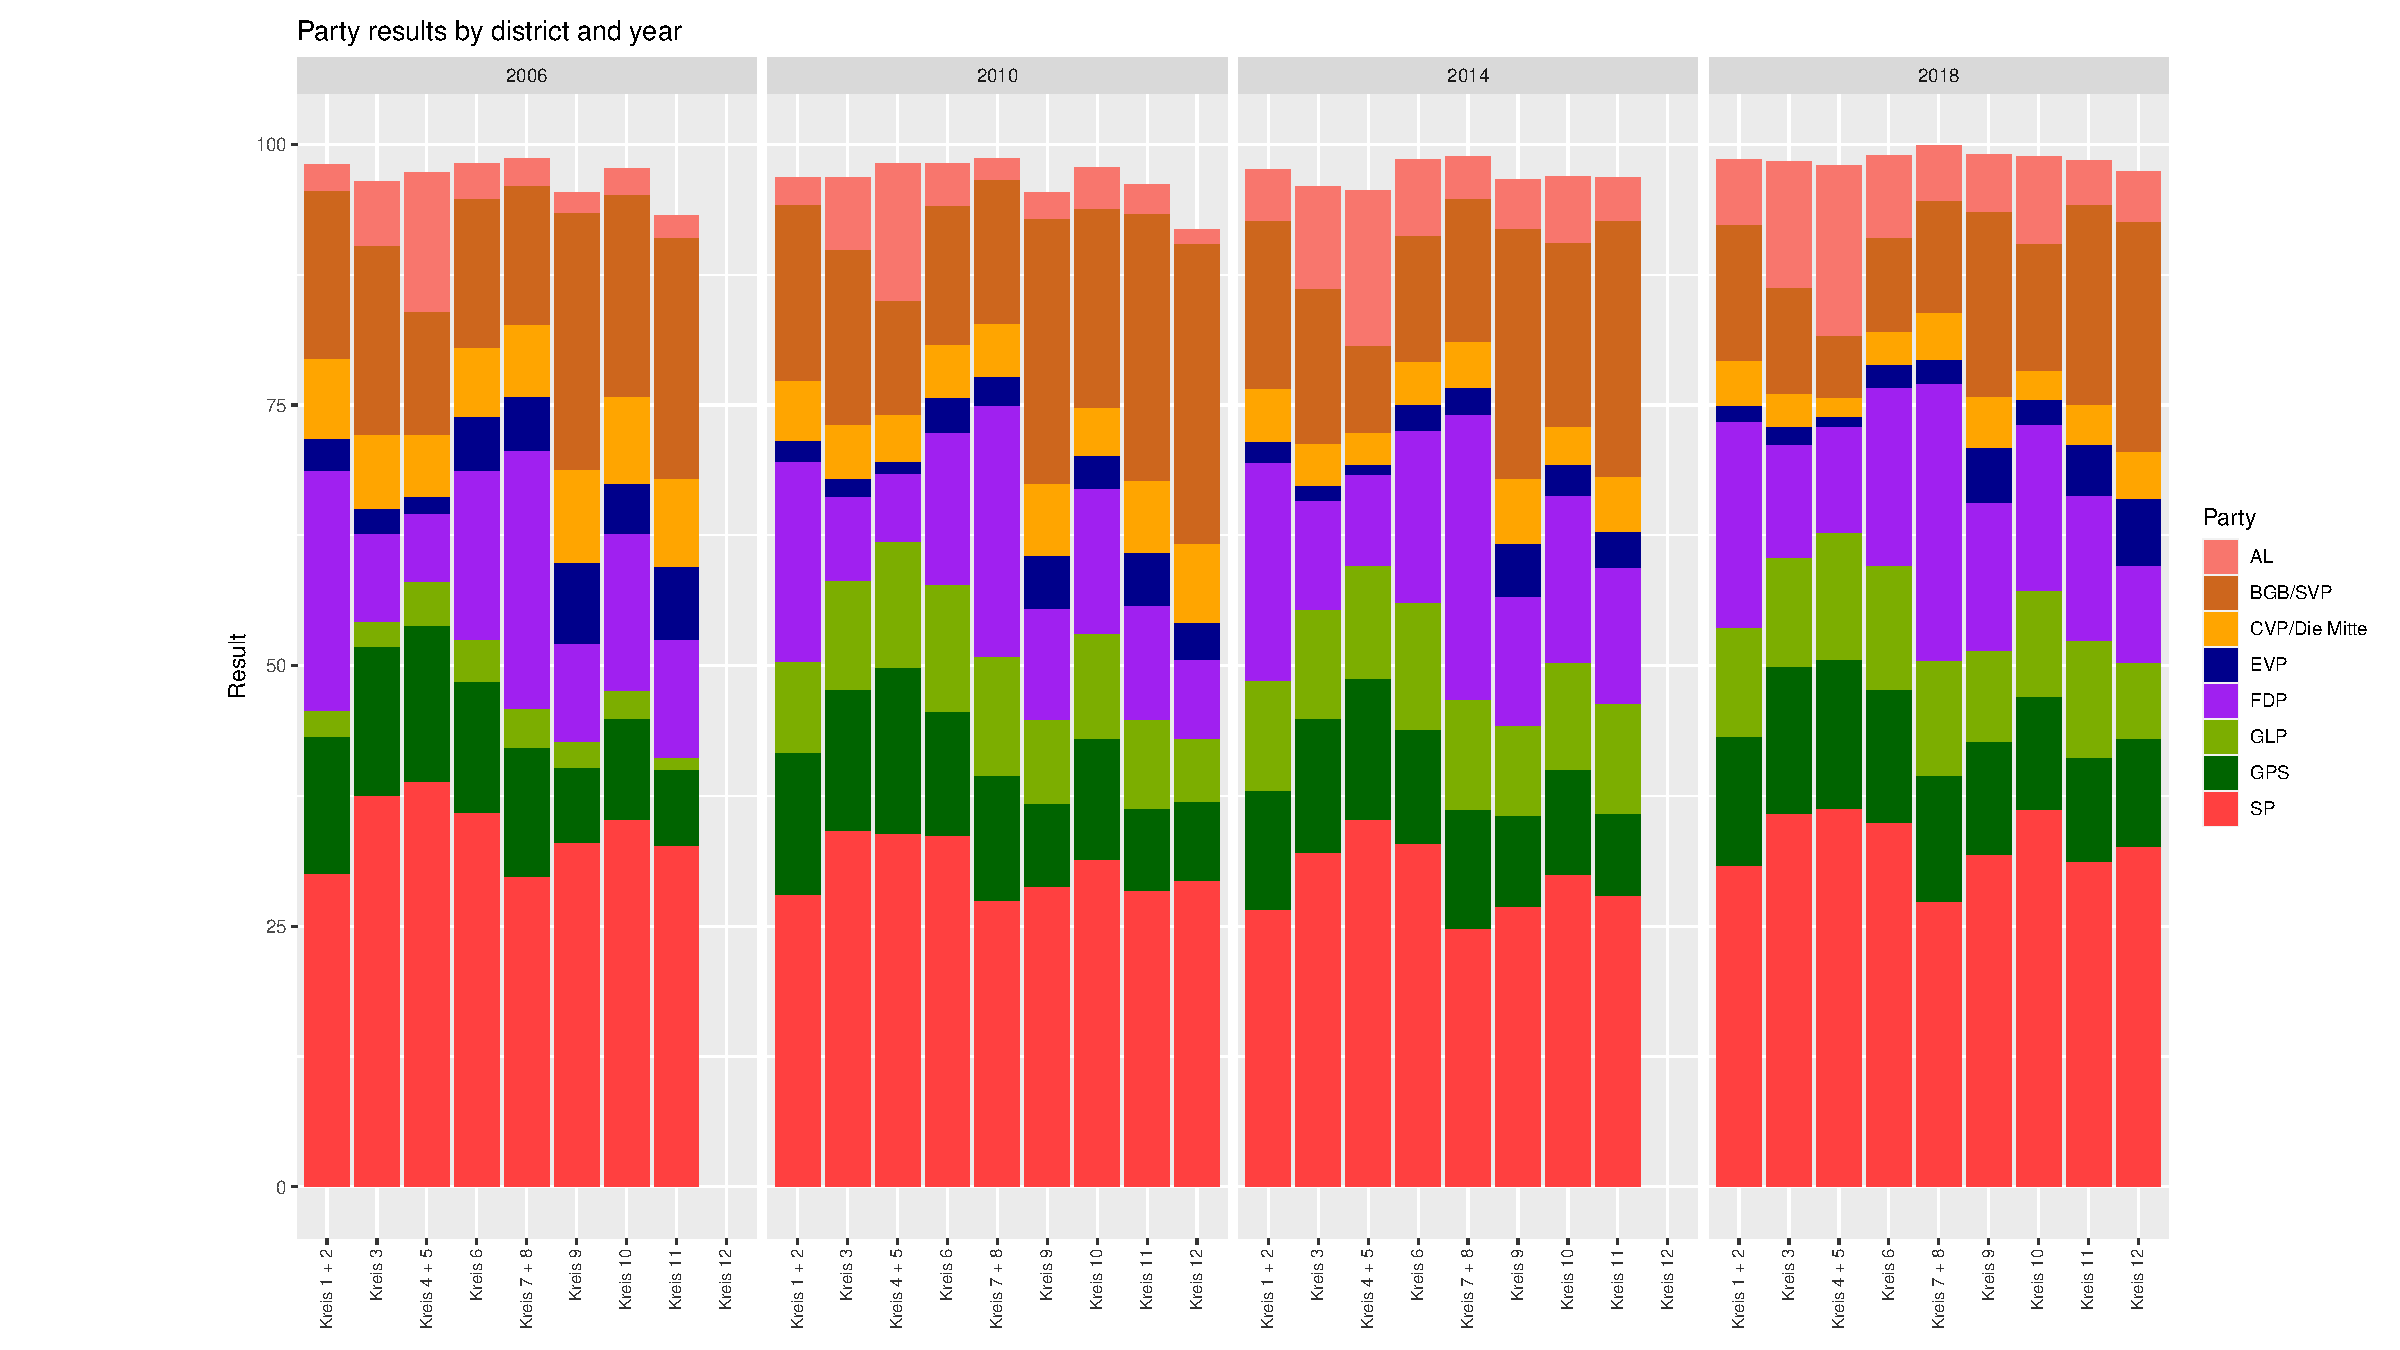
\includegraphics{report_files/figure-latex/plot Parties in Districts-1.pdf}

The data set was merged with the Dataset 1:

\begin{longtable}[]{@{}llrrrrrrrrr@{}}
\caption{Merged dataset: Municipal elections turnout and vote share by
party, 2006-2018.}\tabularnewline
\toprule
Year & DistrictName & PercentageOfDistrict & SP & BGB/SVP & FDP & GPS &
GLP & CVP/Die Mitte & AL & EVP\tabularnewline
\midrule
\endfirsthead
\toprule
Year & DistrictName & PercentageOfDistrict & SP & BGB/SVP & FDP & GPS &
GLP & CVP/Die Mitte & AL & EVP\tabularnewline
\midrule
\endhead
2018 & Kreis 1 + 2 & 55.46 & 30.8 & 13.1 & 19.8 & 12.4 & 10.4 & 4.3 &
6.3 & 1.5\tabularnewline
2018 & Kreis 3 & 58.23 & 35.8 & 10.3 & 10.9 & 14.1 & 10.4 & 3.2 & 12.1 &
1.6\tabularnewline
2018 & Kreis 4 + 5 & 58.24 & 36.3 & 6.1 & 10.2 & 14.3 & 12.1 & 1.8 &
16.3 & 0.9\tabularnewline
2018 & Kreis 6 & 66.55 & 34.9 & 9.1 & 17.2 & 12.8 & 11.8 & 3.2 & 7.8 &
2.1\tabularnewline
2018 & Kreis 7 + 8 & 65.16 & 27.4 & 10.8 & 26.7 & 12.1 & 10.9 & 4.5 &
5.3 & 2.2\tabularnewline
2018 & Kreis 9 & 54.20 & 31.9 & 17.9 & 14.2 & 10.8 & 8.7 & 4.9 & 5.4 &
5.2\tabularnewline
2018 & Kreis 10 & 64.20 & 36.2 & 12.3 & 16.0 & 10.8 & 10.1 & 2.8 & 8.3 &
2.3\tabularnewline
2018 & Kreis 11 & 51.07 & 31.2 & 19.2 & 14.0 & 10.0 & 11.1 & 3.9 & 4.3 &
4.8\tabularnewline
\bottomrule
\end{longtable}

\pagebreak

\hypertarget{data-set-3-wealth-distribution-of-the-population-in-zuxfcrich-by-district}{%
\subsection{Data set 3: Wealth distribution of the population in Zürich,
by
district}\label{data-set-3-wealth-distribution-of-the-population-in-zuxfcrich-by-district}}

The data set of dimensions 756x8 variables reflects how the wealth
distribution in absolute terms changed over time per district and per
tax class. The following table shows the accumulated wealth distribution
across all districts of the city of Zürich between the years 1999 and
2019.

\begin{longtable}[]{@{}rrlr@{}}
\caption{Original data set: Distribution wealth tax per category,
district and year}\tabularnewline
\toprule
SteuerJahr & KreisSort & KreisLang & SteuerTarifSort\tabularnewline
\midrule
\endfirsthead
\toprule
SteuerJahr & KreisSort & KreisLang & SteuerTarifSort\tabularnewline
\midrule
\endhead
1999 & 1 & Kreis 1 & 0\tabularnewline
1999 & 1 & Kreis 1 & 1\tabularnewline
1999 & 1 & Kreis 1 & 2\tabularnewline
1999 & 2 & Kreis 2 & 0\tabularnewline
1999 & 2 & Kreis 2 & 1\tabularnewline
1999 & 2 & Kreis 2 & 2\tabularnewline
\bottomrule
\end{longtable}

\begin{longtable}[]{@{}rlrrr@{}}
\toprule
\begin{minipage}[b]{(\columnwidth - 4\tabcolsep) * \real{0.16}}\raggedleft
SteuerTarifSort\strut
\end{minipage} &
\begin{minipage}[b]{(\columnwidth - 4\tabcolsep) * \real{0.23}}\raggedright
SteuerTarifLang\strut
\end{minipage} &
\begin{minipage}[b]{(\columnwidth - 4\tabcolsep) * \real{0.20}}\raggedleft
SteuerVermoegen\_p50\strut
\end{minipage} &
\begin{minipage}[b]{(\columnwidth - 4\tabcolsep) * \real{0.20}}\raggedleft
SteuerVermoegen\_p25\strut
\end{minipage} &
\begin{minipage}[b]{(\columnwidth - 4\tabcolsep) * \real{0.20}}\raggedleft
SteuerVermoegen\_p75\strut
\end{minipage}\tabularnewline
\midrule
\endhead
\begin{minipage}[t]{(\columnwidth - 4\tabcolsep) * \real{0.16}}\raggedleft
0\strut
\end{minipage} &
\begin{minipage}[t]{(\columnwidth - 4\tabcolsep) * \real{0.23}}\raggedright
Grundtarif\strut
\end{minipage} &
\begin{minipage}[t]{(\columnwidth - 4\tabcolsep) * \real{0.20}}\raggedleft
23.0\strut
\end{minipage} &
\begin{minipage}[t]{(\columnwidth - 4\tabcolsep) * \real{0.20}}\raggedleft
0\strut
\end{minipage} &
\begin{minipage}[t]{(\columnwidth - 4\tabcolsep) * \real{0.20}}\raggedleft
174\strut
\end{minipage}\tabularnewline
\begin{minipage}[t]{(\columnwidth - 4\tabcolsep) * \real{0.16}}\raggedleft
1\strut
\end{minipage} &
\begin{minipage}[t]{(\columnwidth - 4\tabcolsep) * \real{0.23}}\raggedright
Verheiratetentarif\strut
\end{minipage} &
\begin{minipage}[t]{(\columnwidth - 4\tabcolsep) * \real{0.20}}\raggedleft
182.0\strut
\end{minipage} &
\begin{minipage}[t]{(\columnwidth - 4\tabcolsep) * \real{0.20}}\raggedleft
22\strut
\end{minipage} &
\begin{minipage}[t]{(\columnwidth - 4\tabcolsep) * \real{0.20}}\raggedleft
711\strut
\end{minipage}\tabularnewline
\begin{minipage}[t]{(\columnwidth - 4\tabcolsep) * \real{0.16}}\raggedleft
2\strut
\end{minipage} &
\begin{minipage}[t]{(\columnwidth - 4\tabcolsep) * \real{0.23}}\raggedright
Einelternfamilientarif\strut
\end{minipage} &
\begin{minipage}[t]{(\columnwidth - 4\tabcolsep) * \real{0.20}}\raggedleft
27.5\strut
\end{minipage} &
\begin{minipage}[t]{(\columnwidth - 4\tabcolsep) * \real{0.20}}\raggedleft
0\strut
\end{minipage} &
\begin{minipage}[t]{(\columnwidth - 4\tabcolsep) * \real{0.20}}\raggedleft
283\strut
\end{minipage}\tabularnewline
\begin{minipage}[t]{(\columnwidth - 4\tabcolsep) * \real{0.16}}\raggedleft
0\strut
\end{minipage} &
\begin{minipage}[t]{(\columnwidth - 4\tabcolsep) * \real{0.23}}\raggedright
Grundtarif\strut
\end{minipage} &
\begin{minipage}[t]{(\columnwidth - 4\tabcolsep) * \real{0.20}}\raggedleft
37.0\strut
\end{minipage} &
\begin{minipage}[t]{(\columnwidth - 4\tabcolsep) * \real{0.20}}\raggedleft
3\strut
\end{minipage} &
\begin{minipage}[t]{(\columnwidth - 4\tabcolsep) * \real{0.20}}\raggedleft
186\strut
\end{minipage}\tabularnewline
\begin{minipage}[t]{(\columnwidth - 4\tabcolsep) * \real{0.16}}\raggedleft
1\strut
\end{minipage} &
\begin{minipage}[t]{(\columnwidth - 4\tabcolsep) * \real{0.23}}\raggedright
Verheiratetentarif\strut
\end{minipage} &
\begin{minipage}[t]{(\columnwidth - 4\tabcolsep) * \real{0.20}}\raggedleft
148.0\strut
\end{minipage} &
\begin{minipage}[t]{(\columnwidth - 4\tabcolsep) * \real{0.20}}\raggedleft
33\strut
\end{minipage} &
\begin{minipage}[t]{(\columnwidth - 4\tabcolsep) * \real{0.20}}\raggedleft
458\strut
\end{minipage}\tabularnewline
\begin{minipage}[t]{(\columnwidth - 4\tabcolsep) * \real{0.16}}\raggedleft
2\strut
\end{minipage} &
\begin{minipage}[t]{(\columnwidth - 4\tabcolsep) * \real{0.23}}\raggedright
Einelternfamilientarif\strut
\end{minipage} &
\begin{minipage}[t]{(\columnwidth - 4\tabcolsep) * \real{0.20}}\raggedleft
7.0\strut
\end{minipage} &
\begin{minipage}[t]{(\columnwidth - 4\tabcolsep) * \real{0.20}}\raggedleft
0\strut
\end{minipage} &
\begin{minipage}[t]{(\columnwidth - 4\tabcolsep) * \real{0.20}}\raggedleft
61\strut
\end{minipage}\tabularnewline
\bottomrule
\end{longtable}

Examinating the previous showed data revealed that the data set contains
a lot of irrelevant information. For example, the columns
\emph{``KreisSort''} and \emph{``KreisLang''} are redundant, since the
first in simply the encoding of the second in number. The same applies
for the the columns \emph{``SteuerTarifSort''} and
\emph{``SteuerTarifLang''}, since the first here again, is the encoding
of the second in number. However, the columns \emph{``KreisLang''} and
\emph{``SteuerTarifLang''} are redundant and therefore, droped. For
practical reasons the columns \emph{``SteuerVermoegen\_p25''} and
\emph{``SteuerVermoegen\_p75''} were droped as well.\\
Moreover, the columns \emph{``SteuerTarifSort''} and
\emph{``KreisSort''} are converted to factors, since those columns are
automatically defined as integer number. Additionally, the names of the
columns do not correspond with the previous data set and therefore, we
have to change the following:

\begin{longtable}[]{@{}ll@{}}
\toprule
Original Column Name & New Column Name\tabularnewline
\midrule
\endhead
KreisSort & DistrictNumber\tabularnewline
SteuerJahr & Year\tabularnewline
SteuerVermoegen\_p50 & Wealth\tabularnewline
SteuerTarifSort & Category\tabularnewline
\bottomrule
\end{longtable}

Finally, after all modifications, the data set looks as follows:

\begin{longtable}[]{@{}rllr@{}}
\caption{Final data set: Distribution wealth tax per category, district
and year}\tabularnewline
\toprule
Year & DistrictNumber & TaxCategory & Wealth\tabularnewline
\midrule
\endfirsthead
\toprule
Year & DistrictNumber & TaxCategory & Wealth\tabularnewline
\midrule
\endhead
1999 & 1 & 0 & 23.0\tabularnewline
1999 & 1 & 1 & 182.0\tabularnewline
1999 & 1 & 2 & 27.5\tabularnewline
1999 & 2 & 0 & 37.0\tabularnewline
1999 & 2 & 1 & 148.0\tabularnewline
1999 & 2 & 2 & 7.0\tabularnewline
\bottomrule
\end{longtable}

The next graph shows the distribution of wealth per year, tax category
and district in Zurich.

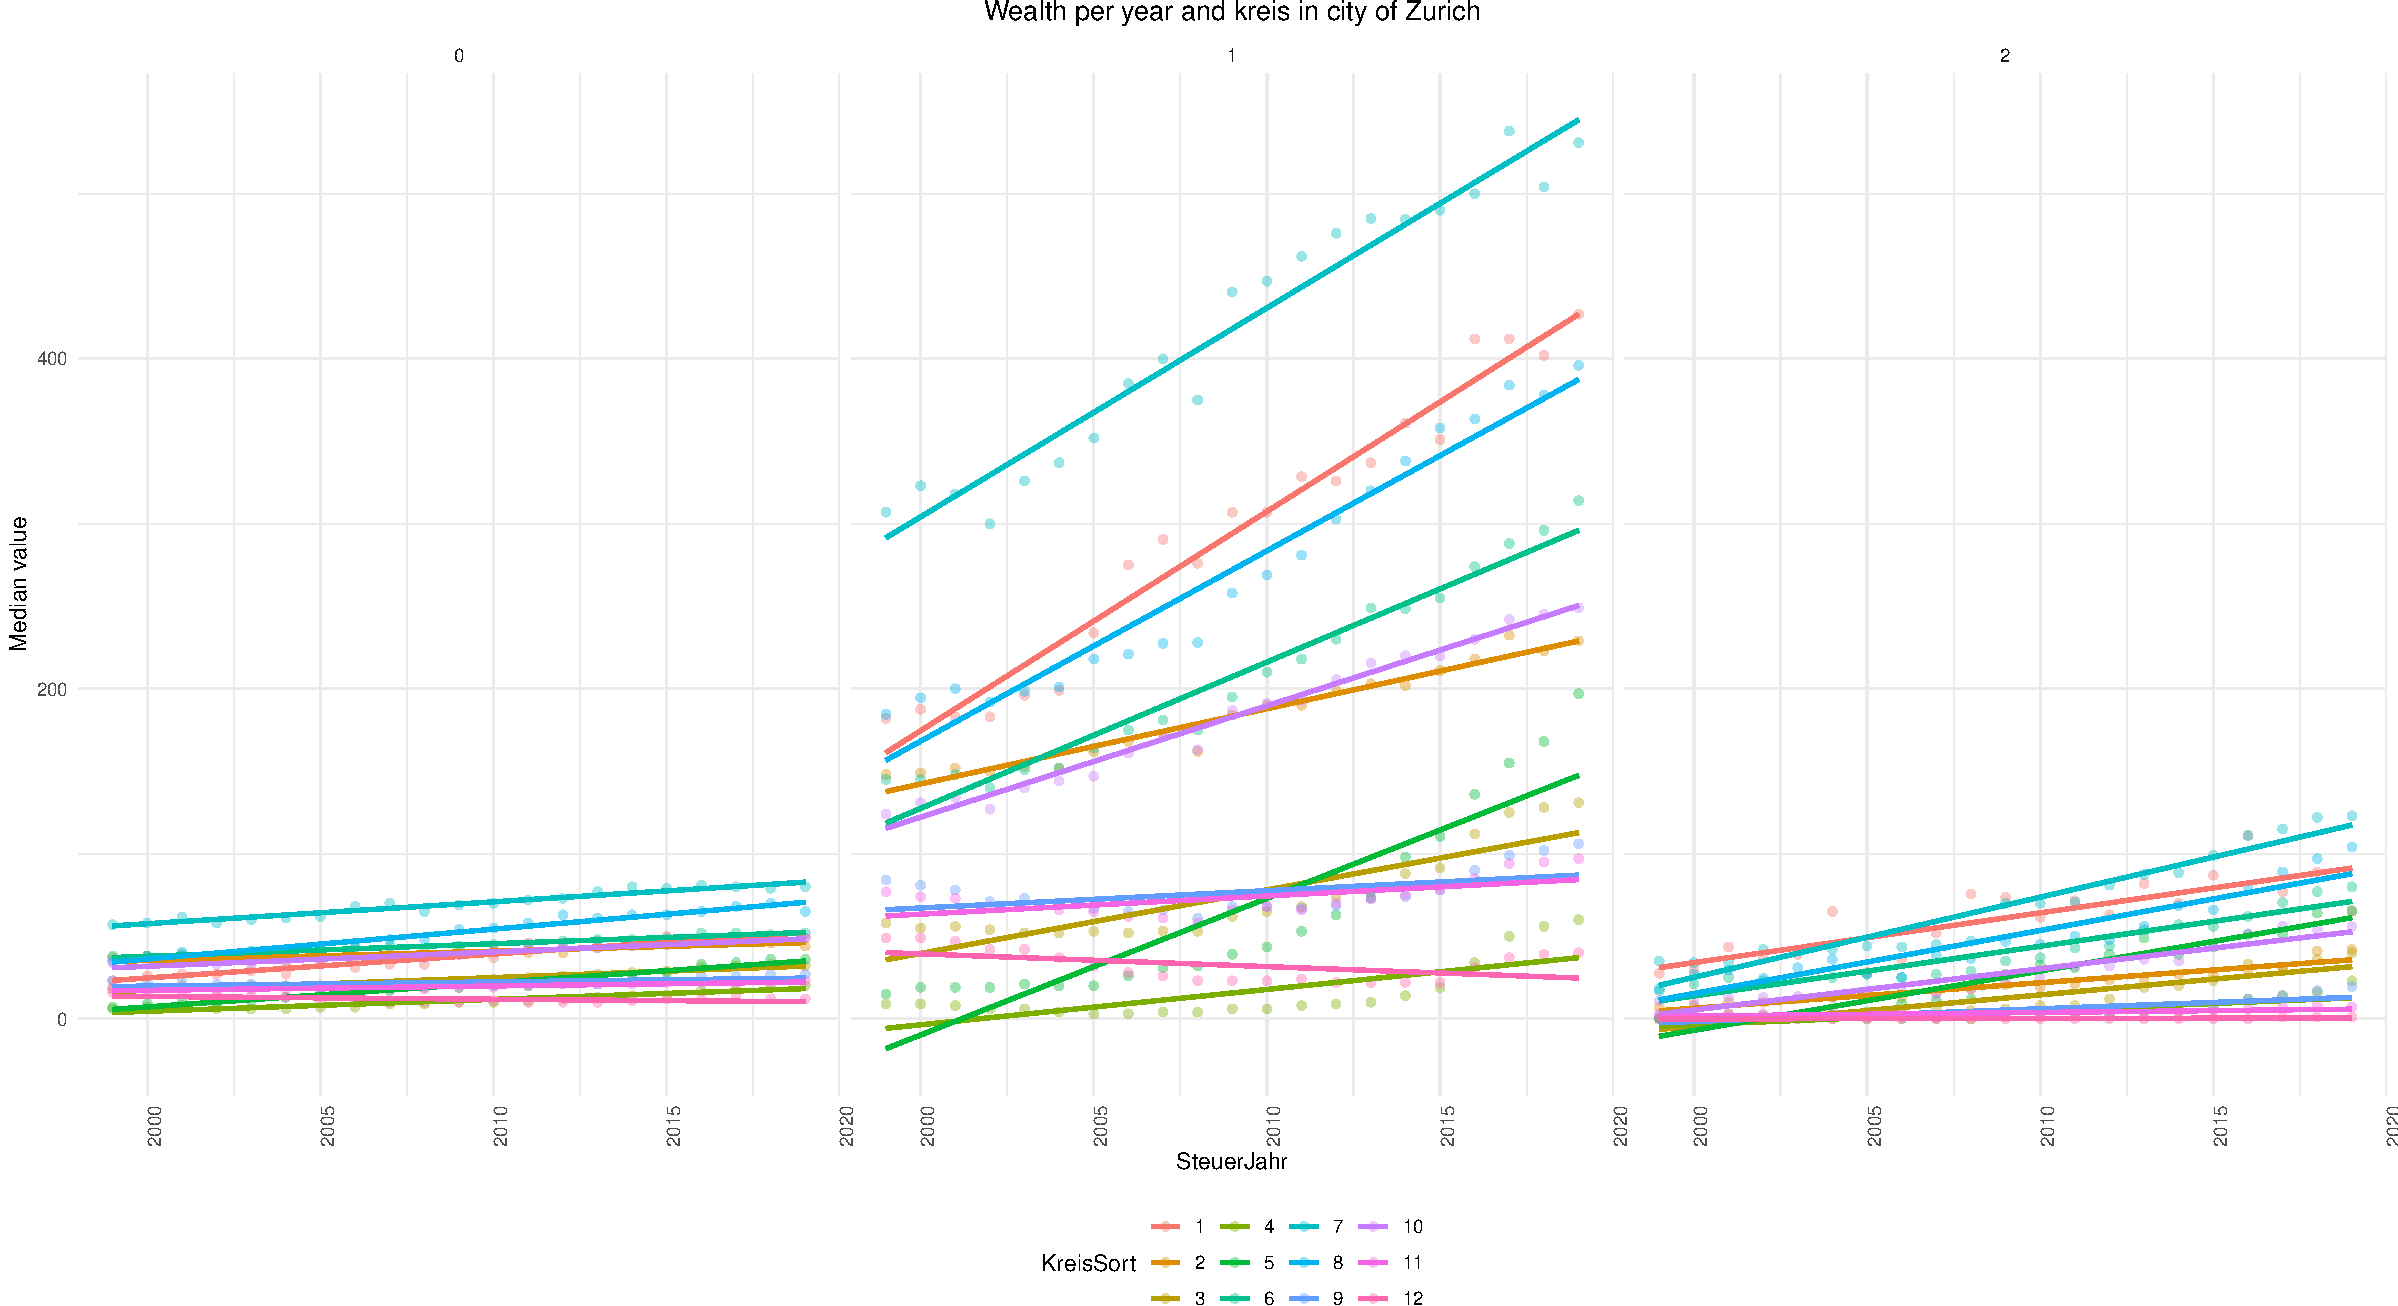
\includegraphics{report_files/figure-latex/plot_wealth-1.pdf}

The previous graph shows the distribution of wealth by district, year
and tax category. Since the ordinate is scaled for all tax categories
with the same values, it is clearly visible the difference of
accumulated wealth between the districts across all and those
differences seems to have a clear trend in increasing. The biggest
differences between districts can be see in the \emph{family category}
subgraph. The highest values have been observed for district 7 and the
lowest values for district 12. District 7, however, has the highest
values among all tax categories. District 12 shows as well across all
categories the lowest values of accumulated as well.

\hypertarget{data-set-4-income-distribution-of-the-population-in-zuxfcrich-by-district}{%
\subsection{Data set 4: Income distribution of the population in Zürich,
by
district}\label{data-set-4-income-distribution-of-the-population-in-zuxfcrich-by-district}}

The following data set of dimensions 756x8 variables reflects how the
income distribution in absolute terms changed over time per district and
per tax class. The following table shows the accumulated income
distribution across all districts of the city of Zürich between the
years 1999 and 2019.

\begin{longtable}[]{@{}rrlr@{}}
\caption{Original data set: Distribution income tax per category,
district and year}\tabularnewline
\toprule
SteuerJahr & KreisSort & KreisLang & SteuerTarifSort\tabularnewline
\midrule
\endfirsthead
\toprule
SteuerJahr & KreisSort & KreisLang & SteuerTarifSort\tabularnewline
\midrule
\endhead
1999 & 1 & Kreis 1 & 0\tabularnewline
1999 & 1 & Kreis 1 & 1\tabularnewline
1999 & 1 & Kreis 1 & 2\tabularnewline
1999 & 2 & Kreis 2 & 0\tabularnewline
1999 & 2 & Kreis 2 & 1\tabularnewline
1999 & 2 & Kreis 2 & 2\tabularnewline
\bottomrule
\end{longtable}

\begin{longtable}[]{@{}lrrr@{}}
\toprule
SteuerTarifLang & SteuerEinkommen\_p50 & SteuerEinkommen\_p25 &
SteuerEinkommen\_p75\tabularnewline
\midrule
\endhead
Grundtarif & 37.8 & 17.40 & 64.80\tabularnewline
Verheiratetentarif & 83.4 & 52.00 & 130.20\tabularnewline
Einelternfamilientarif & 46.7 & 26.05 & 87.05\tabularnewline
Grundtarif & 37.9 & 19.90 & 58.20\tabularnewline
Verheiratetentarif & 69.7 & 49.10 & 101.40\tabularnewline
Einelternfamilientarif & 39.2 & 21.90 & 58.90\tabularnewline
\bottomrule
\end{longtable}

Examinating the previous showed data revealed that the data set contains
a lot of irrelevant information. For example, the columns
\emph{``KreisSort''} and \emph{``KreisLang''} are redundant, since the
first in simply the encoding of the second in number. The same applies
for the the columns \emph{``SteuerTarifSort''} and
\emph{``SteuerTarifLang''}, since the first column, here again, is the
encoding of the second in number. However, the columns
\emph{``KreisLang''} and \emph{``SteuerTarifLang''} are redundant and
therefore, droped. For practical reasons the columns
\emph{``SteuerEinkommen\_p25''} and \emph{``SteuerEinkommen\_p75''} were
droped as well.\\
Moreover, the columns \emph{``SteuerTarifSort''} and
\emph{``KreisSort''} are converted to factors, since those columns are
automatically defined as integer number. Additionally, the names of the
columns do not correspond with the previous data set and therefore, we
have to change the following:

\begin{longtable}[]{@{}ll@{}}
\toprule
Original Column Name & New Column Name\tabularnewline
\midrule
\endhead
KreisSort & DistrictNumber\tabularnewline
SteuerJahr & Year\tabularnewline
SteuerEinkommen\_p50 & Income\tabularnewline
SteuerTarifSort & Category\tabularnewline
\bottomrule
\end{longtable}

Finally, after all modifications, the data set looks as follows:

\begin{longtable}[]{@{}rllr@{}}
\caption{Final data set: Distribution income tax per category, district
and year}\tabularnewline
\toprule
Year & DistrictNumber & TaxCategory & Income\tabularnewline
\midrule
\endfirsthead
\toprule
Year & DistrictNumber & TaxCategory & Income\tabularnewline
\midrule
\endhead
1999 & 1 & 0 & 37.8\tabularnewline
1999 & 1 & 1 & 83.4\tabularnewline
1999 & 1 & 2 & 46.7\tabularnewline
1999 & 2 & 0 & 37.9\tabularnewline
1999 & 2 & 1 & 69.7\tabularnewline
1999 & 2 & 2 & 39.2\tabularnewline
\bottomrule
\end{longtable}

The next graph shows the distribution of income per year, tax category
and district in Zurich.

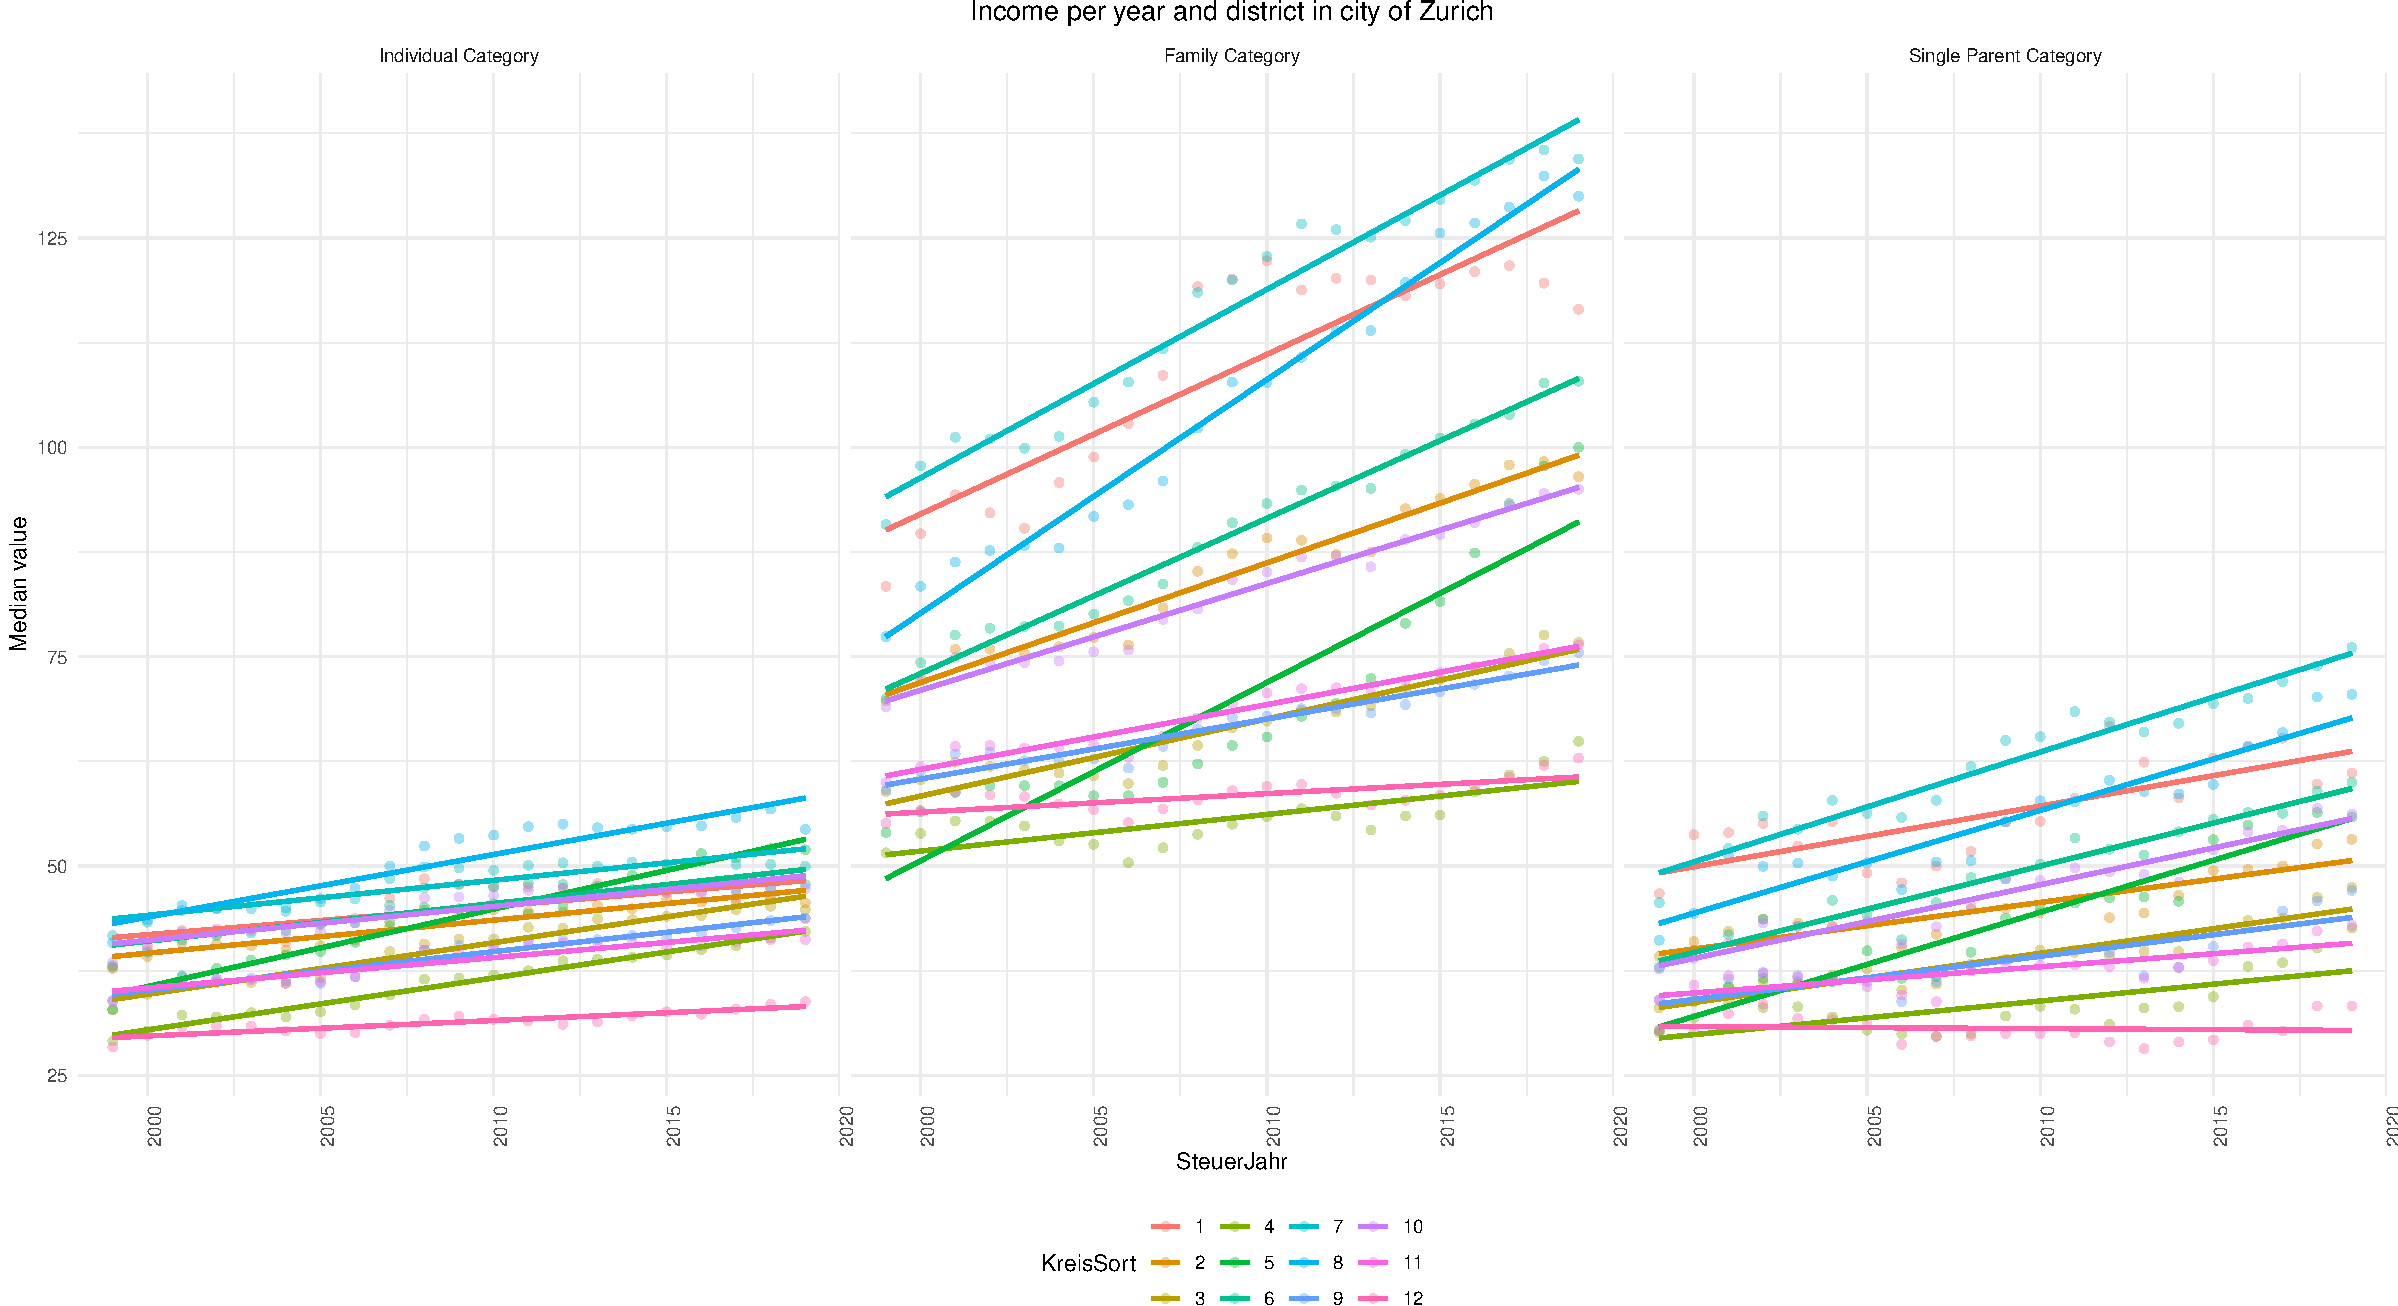
\includegraphics{report_files/figure-latex/plot_income-1.pdf}

The previous graph shows the distribution of income by district, year
and tax category. Since the ordinate is scaled for all tax categories
with the same values, it is clearly visible the difference of
accumulated income between the districts across all and those
differences seems to have a clear trend in increasing. The biggest
differences between districts can be see in the \emph{family category}
subgraph. The highest values have been observed for district 7 and the
lowest values for district 12. District 7, however, has the highest
values among all tax categories. District 12 shows as well across all
categories the lowest values of accumulated as well.

\newpage

\hypertarget{education-data}{%
\subsection{Education data}\label{education-data}}

The following data set contains 39x5 variables on type of education and
year of the complete city of Zürich. This data set allows us to try to
infer the change in education per type in the city of Zürich and
interpolate the change of education type on a district respectively on a
neighborhood level.

\begin{longtable}[]{@{}rlrrr@{}}
\caption{Original data set: Education distribution per category and
year}\tabularnewline
\toprule
Jahr & Bildungsstand & AntBev & untAntBevKI & obAntBevKI\tabularnewline
\midrule
\endfirsthead
\toprule
Jahr & Bildungsstand & AntBev & untAntBevKI & obAntBevKI\tabularnewline
\midrule
\endhead
1970 & Obligatorische Schule & 32.0 & NA & NA\tabularnewline
1970 & Sekundarstufe II & 58.4 & NA & NA\tabularnewline
1970 & Tertiärstufe & 9.7 & NA & NA\tabularnewline
1980 & Obligatorische Schule & 33.9 & NA & NA\tabularnewline
1980 & Sekundarstufe II & 52.5 & NA & NA\tabularnewline
1980 & Tertiärstufe & 13.6 & NA & NA\tabularnewline
\bottomrule
\end{longtable}

The following graphs shows the change of education in the city of Zürich
between the year 1970 and 2018.

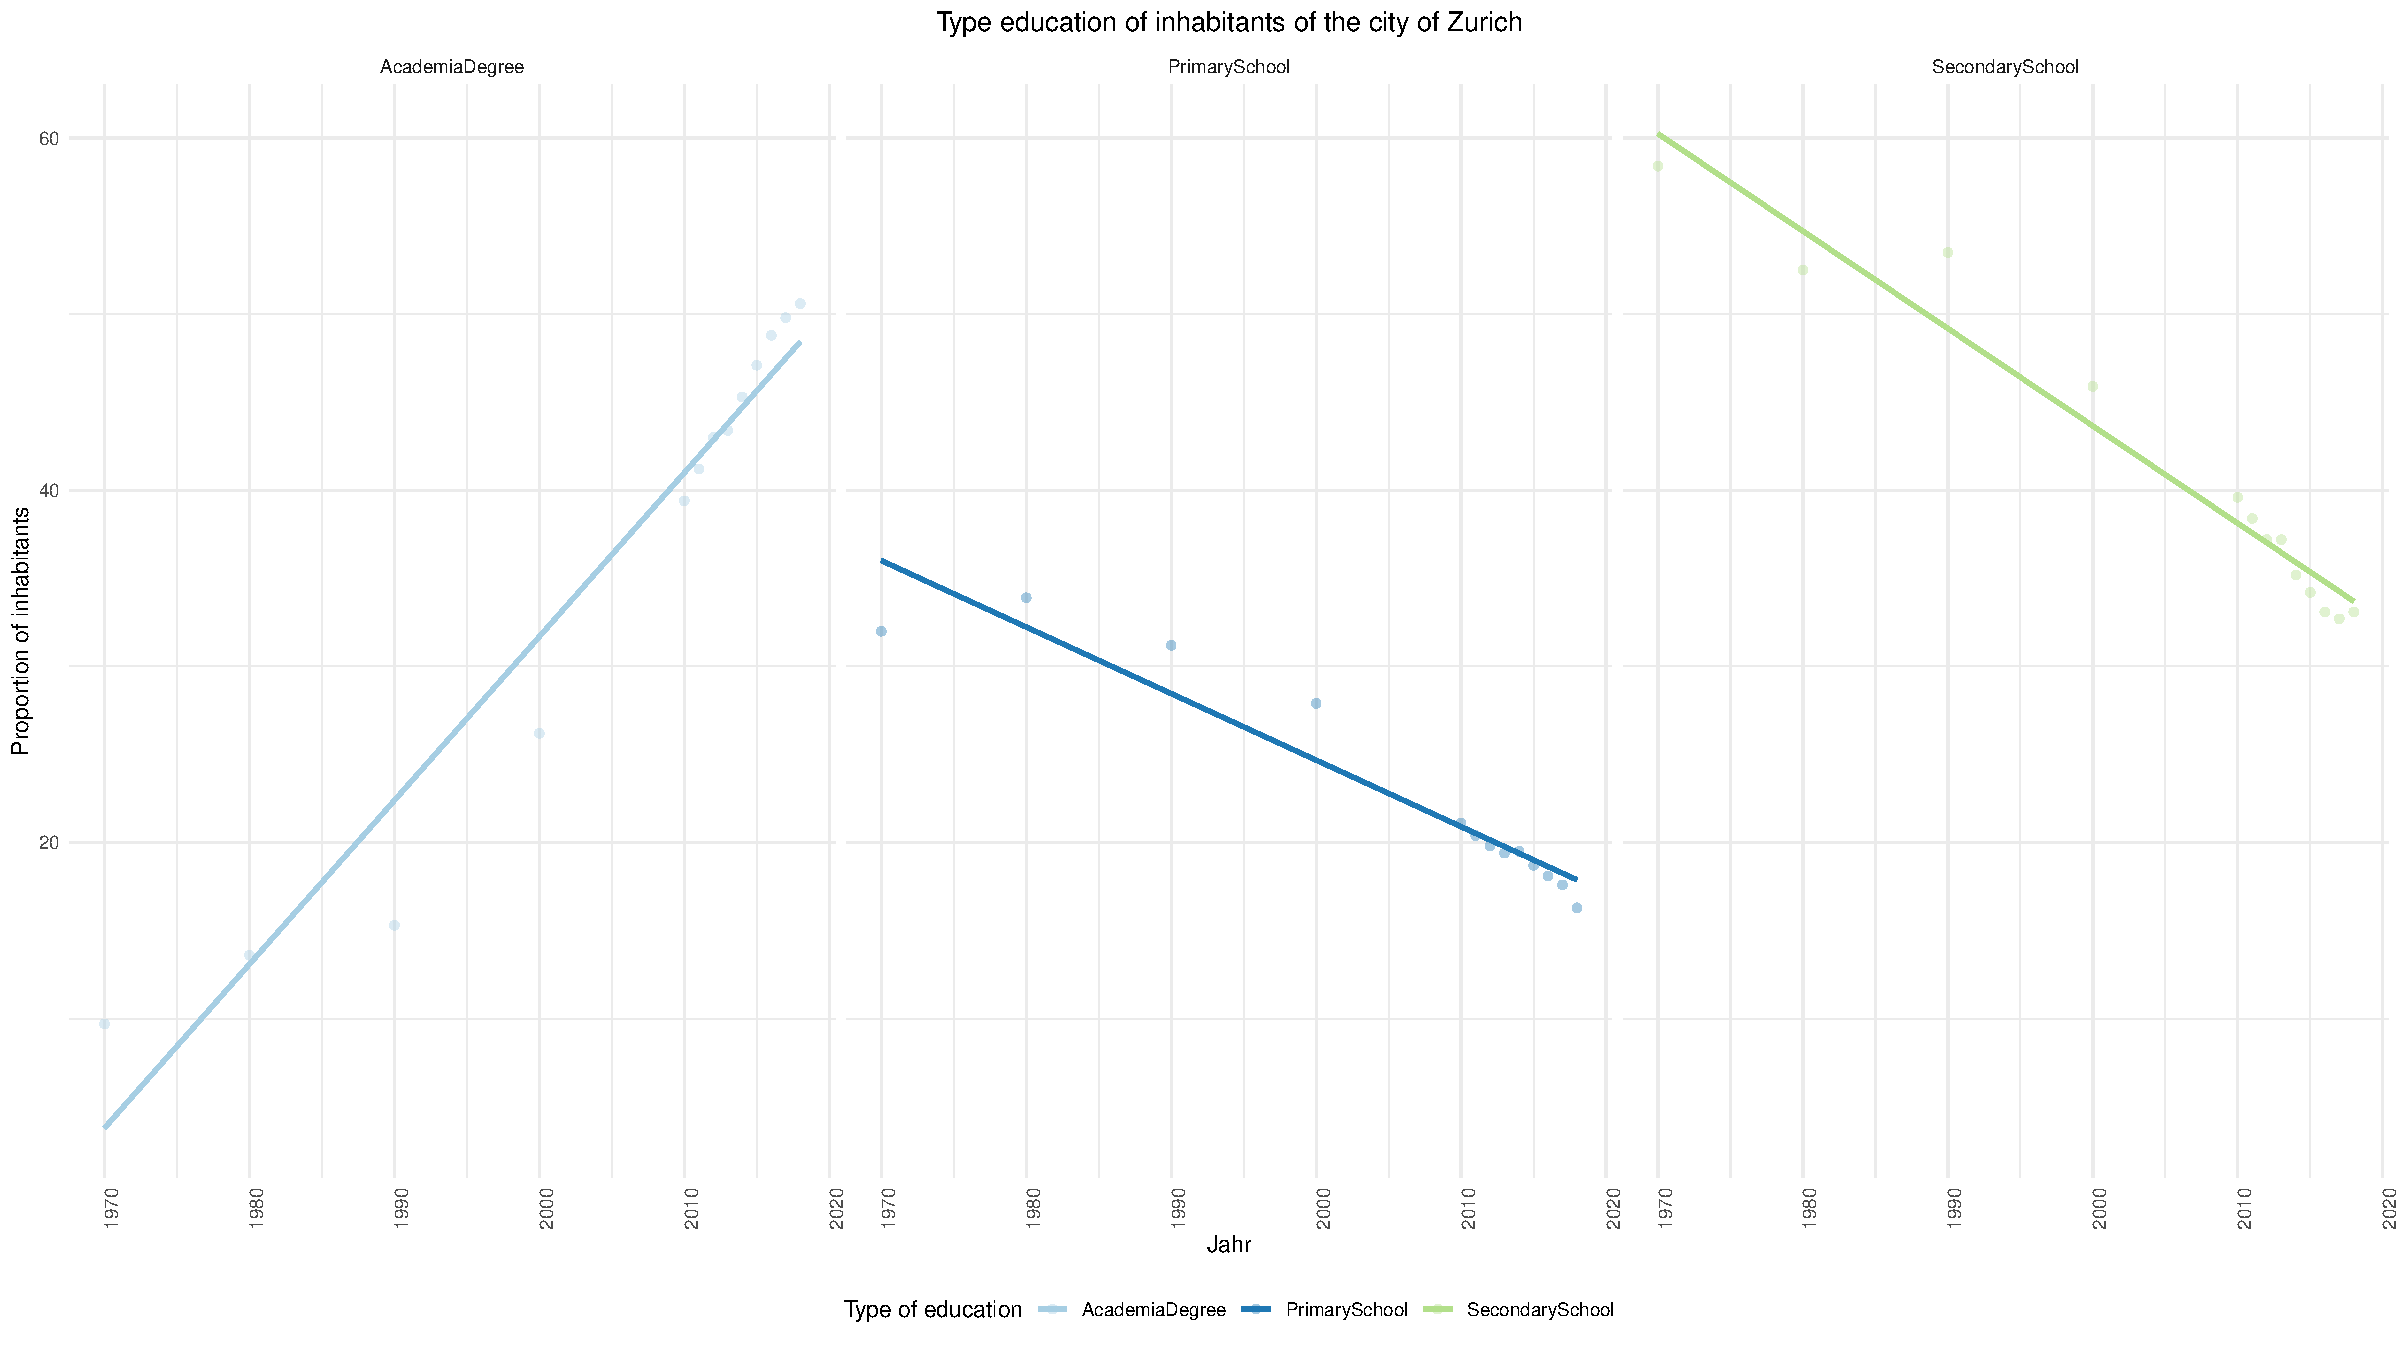
\includegraphics{report_files/figure-latex/plot_education-1.pdf}

The previous graph shows, that the number of inhabitants without an
academical degree is decreasing in the course of time since 1970 in the
City of Zürich, while the number of persons having a university degree
is increasing. First, the values of the previous data frame have to be
re-arranged using the \emph{pivot\_wide()} and the names of the
education type are renamed to match the correspondence table

\begin{longtable}[]{@{}rrrrr@{}}
\caption{Pivoted data set: Education distribution per category and
year}\tabularnewline
\toprule
Year & PrimarySchool & SecondarySchool & AcademiaDegree &
DeltaYear\tabularnewline
\midrule
\endfirsthead
\toprule
Year & PrimarySchool & SecondarySchool & AcademiaDegree &
DeltaYear\tabularnewline
\midrule
\endhead
1970 & 32.0 & 58.4 & 9.7 & 0\tabularnewline
1980 & 33.9 & 52.5 & 13.6 & 10\tabularnewline
1990 & 31.2 & 53.5 & 15.3 & 20\tabularnewline
2000 & 27.9 & 45.9 & 26.2 & 30\tabularnewline
2010 & 21.1 & 39.6 & 39.4 & 40\tabularnewline
2011 & 20.4 & 38.4 & 41.2 & 41\tabularnewline
\bottomrule
\end{longtable}

In order to be able to reproduce this phenomena in the previous data
set, the parameters of theses changes is going to calculated using the
\emph{lm()} function. The used formula is the following:

\[N_{AntBev} = c + \frac{\Delta d_{i}}{\Delta t} \cdot t \]

Applying the previous showed formula to the other data set one gets the
following values

\begin{longtable}[]{@{}lrrr@{}}
\caption{Coefficients of the linear model depending on the education
type}\tabularnewline
\toprule
& PrimarySchool & SecondarySchool & AcademiaDegree\tabularnewline
\midrule
\endfirsthead
\toprule
& PrimarySchool & SecondarySchool & AcademiaDegree\tabularnewline
\midrule
\endhead
(Intercept) & 36.0127064 & 60.240920 & 3.7915859\tabularnewline
DeltaYear & -0.3777745 & -0.552921 & 0.9300644\tabularnewline
\bottomrule
\end{longtable}

The previous table shows the coefficients of the linear model of each
education type. Before further transformation, we load a further data
frame. The data set of dimensions 138x6 variables reflects how the
education of the inhabitants changed over time per district and per
education class. The following table shows the proportion of education
per districts of the city of Zürich for the year 2021. The data set is
updated on a yearly basis.

\begin{longtable}[]{@{}lllrrr@{}}
\caption{Original data set: Education distribution per category and
district for the year 2021}\tabularnewline
\toprule
RaumSort & RaumLang & Bildungsstand & AntBev & untAntBevKI &
obAntBevKI\tabularnewline
\midrule
\endfirsthead
\toprule
RaumSort & RaumLang & Bildungsstand & AntBev & untAntBevKI &
obAntBevKI\tabularnewline
\midrule
\endhead
10 & Kreis 1 & 1 & 9.8 & 6.7 & 12.9\tabularnewline
10 & Kreis 1 & 2 & 26.8 & 22.2 & 31.4\tabularnewline
10 & Kreis 1 & 3 & 63.4 & 58.4 & 68.4\tabularnewline
11 & Rathaus & 1 & 9.9 & 5.9 & 13.9\tabularnewline
11 & Rathaus & 2 & 27.7 & 21.8 & 33.6\tabularnewline
11 & Rathaus & 3 & 62.3 & 55.9 & 68.7\tabularnewline
\bottomrule
\end{longtable}

The column \emph{``RaumSort''} encodes the district number and
corresponding neighborhood within the district. The last digit describes
the neighborhood and the first one (or two) digit the district number.
The column \emph{``RaumLang''} describes the district and neighborhood
name and the column \emph{``Bildungsstand''} describes the type of
education as follows:

\begin{longtable}[]{@{}ll@{}}
\caption{Education ecoding: Education number key vs.~meaning in
words}\tabularnewline
\toprule
EducationNumber & Meaning\tabularnewline
\midrule
\endfirsthead
\toprule
EducationNumber & Meaning\tabularnewline
\midrule
\endhead
1 & Primary school\tabularnewline
2 & Secondary school\tabularnewline
3 & Academia degree\tabularnewline
\bottomrule
\end{longtable}

Where type \emph{1} describes the nine complete year of the mandatory
school program, \emph{2} describes either a professional degree or
high-school diploma and \emph{3} an academical degree (Bachelor's degree
and higher). The columns \emph{``untAntBevKI''} and
\emph{``obAntBevKI''} describes the lower and upper portion of the
confidence interval of the values per education. Summarzing, the data
frame is going to be updated as follows:\\
- \emph{``Bildungsstand''} is update with the meaning as described in
the previous table\\
- Columns \emph{``untAntBevKI''} and \emph{``obAntBevKI''} are droped\\
- Column \emph{``Year''} is added with value \emph{2021}\\
- Column \emph{``RaumSort''} is transformed to column
\emph{``DistrictNumer''}\\
- District designation adapted\\
- District summarized according to voting data frames

Those transformations steps leads to the following data frame:

\begin{longtable}[]{@{}rlrrr@{}}
\caption{Transformed data frame for education in year
2021}\tabularnewline
\toprule
Year & DistrictName & PrimarySchool & SecondarySchool &
AcademiaDegree\tabularnewline
\midrule
\endfirsthead
\toprule
Year & DistrictName & PrimarySchool & SecondarySchool &
AcademiaDegree\tabularnewline
\midrule
\endhead
2021 & Kreis 1 + 2 & 12.5 & 29.7 & 57.8\tabularnewline
2021 & Kreis 10 & 12.4 & 33.7 & 54.0\tabularnewline
2021 & Kreis 11 & 20.3 & 35.5 & 44.2\tabularnewline
2021 & Kreis 12 & 29.2 & 39.6 & 31.1\tabularnewline
2021 & Kreis 3 & 17.2 & 31.6 & 51.2\tabularnewline
2021 & Kreis 4 + 5 & 13.9 & 26.9 & 59.3\tabularnewline
2021 & Kreis 6 & 10.0 & 25.4 & 64.6\tabularnewline
2021 & Kreis 7 + 8 & 8.4 & 26.4 & 65.2\tabularnewline
2021 & Kreis 9 & 20.0 & 38.6 & 41.5\tabularnewline
\bottomrule
\end{longtable}

The previous table shows the transformed data for the year 2021. Now,
taking into account the previously calculated
\emph{\href{tab:pivot_education1}{lm coefficients}} one can extrapolate
values for the missing years of the data frame.

\pagebreak

\hypertarget{merging-data}{%
\section{Merging Data}\label{merging-data}}

\hypertarget{combine-wealth-and-income-data}{%
\subsection{Combine wealth and income
data}\label{combine-wealth-and-income-data}}

The aim of this part is to combine the income and wealth data into one
data frame. As a first step, both data frames are combine using the
\emph{merge()} function. The merged data sets of income and wealth data,
contains the income data and wealth data per district and tax category
combined.

\begin{longtable}[]{@{}rllrr@{}}
\caption{Merged income and wealth data}\tabularnewline
\toprule
Year & DistrictNumber & TaxCategory & Income & Wealth\tabularnewline
\midrule
\endfirsthead
\toprule
Year & DistrictNumber & TaxCategory & Income & Wealth\tabularnewline
\midrule
\endhead
1999 & 1 & 0 & 37.8 & 23.0\tabularnewline
1999 & 1 & 1 & 83.4 & 182.0\tabularnewline
1999 & 1 & 2 & 46.7 & 27.5\tabularnewline
1999 & 10 & 0 & 38.5 & 34.0\tabularnewline
1999 & 10 & 1 & 69.0 & 124.0\tabularnewline
1999 & 10 & 2 & 37.7 & 11.0\tabularnewline
\bottomrule
\end{longtable}

Thereafter, the district name has to be modified in order to match if
the data presented in sections concerning
\emph{\protect\hyperlink{Dataux5cux2520setux5cux25201:ux5cux2520Turnoutux5cux2520atux5cux2520theux5cux2520cityux5cux2520andux5cux2520municipalux5cux2520councilux5cux2520electionsux5cux2520sinceux5cux25202006ux2cux5cux2520byux5cux2520cityux5cux2520district.}{Data
set 1}} and
\emph{\protect\hyperlink{Dataux5cux2520setux5cux25202:ux5cux2520Municipalux5cux2520electionsux5cux2520voteux5cux2520shareux2cux5cux2520byux5cux2520partyux5cux2520andux5cux2520electoralux5cux2520districtux5cux2520sinceux5cux25201913.}{Data
set 2}}: The name of the districts corresponds to the prefix
\emph{``Kreis''} followed by \emph{" + "} and the corresponding number.
In the case of the \emph{wealth} and \emph{income} data frames, those
values have to be transformed and combined as the following
correspondence tables shows:

\begin{longtable}[]{@{}ll@{}}
\caption{Correspondence table between district names and district
numbers}\tabularnewline
\toprule
Number & Name\tabularnewline
\midrule
\endfirsthead
\toprule
Number & Name\tabularnewline
\midrule
\endhead
1 & Kreis 1 + 2\tabularnewline
2 & Kreis 1 + 2\tabularnewline
3 & Kreis 3\tabularnewline
4 & Kreis 4 + 5\tabularnewline
5 & Kreis 4 + 5\tabularnewline
6 & Kreis 6\tabularnewline
7 & Kreis 7 + 8\tabularnewline
8 & Kreis 7 + 8\tabularnewline
9 & Kreis 9\tabularnewline
10 & Kreis 10\tabularnewline
11 & Kreis 11\tabularnewline
12 & Kreis 12\tabularnewline
\bottomrule
\end{longtable}

Thereafter, several transformations have to be done as follows in order
to transform the data into a mergable format:\\
- Pivot to a longer format the tables and combine the tax values\\
- Group by year, district name and tax type\\
- Sum the values amount all categories within one district\\
- Pivot to wide format again to averaged values

After the step-by-step implementation of those transformation steps one
gets the following data frame:

\begin{longtable}[]{@{}rlrr@{}}
\caption{Final wealth and income data frame per district and
year}\tabularnewline
\toprule
Year & DistrictName & SumTaxIncome & SumTaxWealth\tabularnewline
\midrule
\endfirsthead
\toprule
Year & DistrictName & SumTaxIncome & SumTaxWealth\tabularnewline
\midrule
\endhead
1999 & Kreis 1 + 2 & 314.70 & 424.5\tabularnewline
1999 & Kreis 3 & 124.75 & 76.0\tabularnewline
1999 & Kreis 4 + 5 & 228.10 & 37.0\tabularnewline
1999 & Kreis 6 & 146.00 & 200.0\tabularnewline
1999 & Kreis 7 + 8 & 337.55 & 636.5\tabularnewline
1999 & Kreis 9 & 127.15 & 108.0\tabularnewline
\bottomrule
\end{longtable}

\hypertarget{merge-all-data-sets}{%
\subsection{Merge all data sets}\label{merge-all-data-sets}}

Finally, all data sets are combined into one:

\begin{longtable}[]{@{}llrr@{}}
\caption{Final dataset}\tabularnewline
\toprule
Year & DistrictName & SumTaxIncome & SumTaxWealth\tabularnewline
\midrule
\endfirsthead
\toprule
Year & DistrictName & SumTaxIncome & SumTaxWealth\tabularnewline
\midrule
\endhead
2006 & Kreis 1 + 2 & 352.45 & 561.0\tabularnewline
2006 & Kreis 3 & 132.95 & 76.0\tabularnewline
2006 & Kreis 4 + 5 & 249.65 & 61.0\tabularnewline
2006 & Kreis 6 & 166.10 & 243.0\tabularnewline
2006 & Kreis 7 + 8 & 397.45 & 788.5\tabularnewline
2006 & Kreis 9 & 132.30 & 85.5\tabularnewline
\bottomrule
\end{longtable}

\begin{longtable}[]{@{}rrrrrrrrr@{}}
\toprule
PercentageOfDistrict & SP & BGB/SVP & FDP & GPS & GLP & CVP/Die Mitte &
AL & EVP\tabularnewline
\midrule
\endhead
34.96 & 30.1 & 16.2 & 23.1 & 13.1 & 2.4 & 7.7 & 2.5 & 3.0\tabularnewline
33.20 & 37.5 & 18.2 & 8.6 & 14.3 & 2.3 & 7.1 & 6.1 & 2.3\tabularnewline
28.20 & 38.9 & 11.9 & 6.6 & 14.9 & 4.2 & 6.0 & 13.3 & 1.5\tabularnewline
40.75 & 35.9 & 14.4 & 16.3 & 12.6 & 3.9 & 6.6 & 3.4 & 5.1\tabularnewline
39.51 & 29.8 & 13.5 & 24.8 & 12.3 & 3.7 & 6.9 & 2.6 & 5.1\tabularnewline
33.05 & 33.0 & 24.8 & 9.5 & 7.2 & 2.4 & 8.9 & 1.9 & 7.7\tabularnewline
\bottomrule
\end{longtable}

\pagebreak

\hypertarget{chapter-of-choice---maps-with-ggplot-and-sf}{%
\section{Chapter of choice - Maps with ggplot and
sf}\label{chapter-of-choice---maps-with-ggplot-and-sf}}

As a chapter of choice, we have explored creation of maps in ggplot and
sf.

\hypertarget{r-maps-1-echofalse-includefalse}{%
\section{```\{r Maps 1, echo=FALSE,
include=FALSE\}}\label{r-maps-1-echofalse-includefalse}}

\hypertarget{libraryggplot2}{%
\section{library(ggplot2)}\label{libraryggplot2}}

\hypertarget{librarysf}{%
\section{library(sf)}\label{librarysf}}

\hypertarget{libraryosmdata}{%
\section{library(osmdata)}\label{libraryosmdata}}

\hypertarget{libraryggmap}{%
\section{library(ggmap)}\label{libraryggmap}}

\hypertarget{load-files-with-map-information}{%
\section{\#\# Load files with map
information}\label{load-files-with-map-information}}

\hypertarget{zh---st_readusersleonidgavrilyukdesktopr_bootcamprbootcampmap_datastzh.adm_zaehlkreise_a.shp}{%
\section{\#zh \textless-
st\_read(``/Users/leonidgavrilyuk/Desktop/R\_Bootcamp/RBootcamp/map\_data/stzh.adm\_zaehlkreise\_a.shp'')}\label{zh---st_readusersleonidgavrilyukdesktopr_bootcamprbootcampmap_datastzh.adm_zaehlkreise_a.shp}}

\hypertarget{zh---st_readusersleonidgavrilyukdesktopr_bootcamprbootcampmap_datastzh.adm_zaehlkreise_a.shp-1}{%
\section{zh \textless-
st\_read(``/Users/leonidgavrilyuk/Desktop/R\_Bootcamp/RBootcamp/map\_data/stzh.adm\_zaehlkreise\_a.shp'')}\label{zh---st_readusersleonidgavrilyukdesktopr_bootcamprbootcampmap_datastzh.adm_zaehlkreise_a.shp-1}}

\hypertarget{zh---zh}{%
\section{zh \textless- zh \%\textgreater\%}\label{zh---zh}}

\hypertarget{dplyrmutatebezeichnun-recodebezeichnun}{%
\section{dplyr::mutate(bezeichnun =
recode(bezeichnun,}\label{dplyrmutatebezeichnun-recodebezeichnun}}

\hypertarget{kreis-3}{%
\section{``3'' = ``Kreis 3'',}\label{kreis-3}}

\hypertarget{kreis-6}{%
\section{``6'' = ``Kreis 6'',}\label{kreis-6}}

\hypertarget{kreis-910-kreis-10}{%
\section{``9'' = ``Kreis 9'',``10'' = ``Kreis
10'',}\label{kreis-910-kreis-10}}

\hypertarget{kreis-11}{%
\section{``11'' = ``Kreis 11'',}\label{kreis-11}}

\hypertarget{kreis-12}{%
\section{``12'' = ``Kreis 12'',}\label{kreis-12}}

\hypertarget{und-2-kreis-1-2}{%
\section{`1 und 2' = `Kreis 1 + 2',}\label{und-2-kreis-1-2}}

\hypertarget{und-5-kreis-4-5}{%
\section{`4 und 5' = `Kreis 4 + 5',}\label{und-5-kreis-4-5}}

\hypertarget{und-8-kreis-7-8}{%
\section{`7 und 8' =`Kreis 7 + 8'))}\label{und-8-kreis-7-8}}

\hypertarget{zh---zh-1}{%
\section{zh \textless- zh \%\textgreater\%}\label{zh---zh-1}}

\hypertarget{mutatekuerzel-recodekuerzel}{%
\section{mutate(kuerzel =
recode(kuerzel,}\label{mutatekuerzel-recodekuerzel}}

\hypertarget{und-2-12}{%
\section{`1 und 2' = `1+2',}\label{und-2-12}}

\hypertarget{und-5-45}{%
\section{`4 und 5' = `4+5',}\label{und-5-45}}

\hypertarget{und-8-78}{%
\section{`7 und 8' =`7+8'))}\label{und-8-78}}

\hypertarget{zhbezeichnun---factorzhbezeichnun-levels-ckreis-1-2kreis-3}{%
\section{\texorpdfstring{zh\(bezeichnun <- factor(zh\)bezeichnun, levels
= c(``Kreis 1 + 2'',``Kreis
3'',}{zhbezeichnun \textless- factor(zhbezeichnun, levels = c(``Kreis 1 + 2'',``Kreis 3'',}}\label{zhbezeichnun---factorzhbezeichnun-levels-ckreis-1-2kreis-3}}

\hypertarget{kreis-4-5-kreis-6}{%
\section{``Kreis 4 + 5'', ``Kreis 6'',}\label{kreis-4-5-kreis-6}}

\hypertarget{kreis-7-8-kreis-9}{%
\section{`Kreis 7 + 8', ``Kreis 9'',}\label{kreis-7-8-kreis-9}}

\hypertarget{kreis-10}{%
\section{``Kreis 10'',}\label{kreis-10}}

\hypertarget{kreis-11-kreis-12}{%
\section{``Kreis 11'', ``Kreis 12'' ))}\label{kreis-11-kreis-12}}

\hypertarget{zh---zhorderzhbezeichnun}{%
\section{zh \textless-
zh{[}order(zh\$bezeichnun),{]}}\label{zh---zhorderzhbezeichnun}}

\hypertarget{zh---zh-2}{%
\section{zh \textless- zh \%\textgreater\%}\label{zh---zh-2}}

\hypertarget{dplyrrename}{%
\section{dplyr::rename(}\label{dplyrrename}}

\hypertarget{districtname-bezeichnun}{%
\section{DistrictName = bezeichnun}\label{districtname-bezeichnun}}

\hypertarget{section}{%
\section{)}\label{section}}

\hypertarget{results---df_finaldf_finalyear-in-c2018}{%
\section{results \textless- df\_final{[}df\_final\$Year \%in\%
c(``2018''), {]}}\label{results---df_finaldf_finalyear-in-c2018}}

\hypertarget{zh---zh-dplyrinner_joinresults}{%
\section{zh \textless- zh \%\textgreater\%
dplyr::inner\_join(results)}\label{zh---zh-dplyrinner_joinresults}}

\hypertarget{headzh-10}{%
\section{head(zh, 10)}\label{headzh-10}}

\hypertarget{section-1}{%
\section{```}\label{section-1}}

\hypertarget{r-plot-map-include-true-dimzh-ggplotdata-zh-geom_sfaesfill-sp-scale_fill_viridis_ctrans-sqrt-geom_sf_labelaeslabel-kuerzel-colour-white-geom_sf_textaeslabel-kuerzel-colour-black-size2familysans-labsfill-2018-sp-results}{%
\section{\texorpdfstring{\texttt{\{r\ plot\ map,\ include\ =\ TRUE\}\ \#\ dim(zh)\ \#\ ggplot(data\ =\ zh)\ +\ \#\ \ \ geom\_sf(aes(fill\ =\ SP))\ +\ \#\ \ \ scale\_fill\_viridis\_c(trans\ =\ "sqrt")\ +\ \#\ \ \ geom\_sf\_label(aes(label\ =\ kuerzel),\ colour\ =\ "white")\ +\ \#\ \ \ geom\_sf\_text(aes(label\ =\ kuerzel),\ colour\ =\ "black",\ size=2,family="sans")\ +\ \#\ \ \ labs(fill\ =\ "2018\ SP\ results\ (\%)")\ \#\ \#}}{\{r plot map, include = TRUE\} \# dim(zh) \# ggplot(data = zh) + \#   geom\_sf(aes(fill = SP)) + \#   scale\_fill\_viridis\_c(trans = "sqrt") + \#   geom\_sf\_label(aes(label = kuerzel), colour = "white") + \#   geom\_sf\_text(aes(label = kuerzel), colour = "black", size=2,family="sans") + \#   labs(fill = "2018 SP results (\%)") \# \#}}\label{r-plot-map-include-true-dimzh-ggplotdata-zh-geom_sfaesfill-sp-scale_fill_viridis_ctrans-sqrt-geom_sf_labelaeslabel-kuerzel-colour-white-geom_sf_textaeslabel-kuerzel-colour-black-size2familysans-labsfill-2018-sp-results}}

\pagebreak

\hypertarget{data-visualization}{%
\section{Data Visualization}\label{data-visualization}}

\pagebreak

\hypertarget{fit-model}{%
\section{Fit Model}\label{fit-model}}

\pagebreak

\hypertarget{references}{%
\section{References}\label{references}}

\end{document}
